% IntelliRoute --- CMPE 273 Spring 2026
% Compiles cleanly on Overleaf with the default IEEEtran package.
\documentclass[conference,letterpaper]{IEEEtran}

\usepackage{cite}
\usepackage{amsmath}
\usepackage{amssymb}
\usepackage{graphicx}
\usepackage{booktabs}
\usepackage{array}
\usepackage{tabularx}
\usepackage{xcolor}
\usepackage{listings}
\usepackage{tikz}
\usetikzlibrary{arrows.meta,positioning,shapes.geometric,calc,fit,backgrounds}
\usepackage[hidelinks]{hyperref}

% --- listing style for short code references ------------------------------
\lstset{
  basicstyle=\ttfamily\footnotesize,
  columns=fullflexible,
  keepspaces=true,
  breaklines=true,
  frame=single,
  framerule=0.3pt,
  xleftmargin=4pt,
  xrightmargin=4pt,
}

% Tighten spacing a little so the paper stays in the 5-6 page budget.
\setlength{\textfloatsep}{6pt plus 1pt minus 1pt}
\setlength{\intextsep}{6pt plus 1pt minus 1pt}
\setlength{\dbltextfloatsep}{6pt plus 1pt minus 1pt}

\begin{document}

\title{IntelliRoute: A Distributed Control Plane for\\
       Multi-LLM Orchestration}

\author{
\IEEEauthorblockN{Anukrithi Myadala, Larry Nguyen, James Pham, Surbhi Singh}
\IEEEauthorblockA{
  Department of Computer Engineering\\
  San Jos\'e State University\\
  CMPE 273 --- Enterprise Distributed Systems, Spring 2026}
}

\maketitle

\begin{abstract}
Most teams that ship features on top of large language models (LLMs)
end up calling a provider SDK directly from application code, wrapped
in a try/except that retries the same provider once
and then gives up. As soon as a second provider is added, this pattern
collapses: routing logic gets sprinkled across services, quotas are
fragmented per provider, cost arrives in a monthly bill that nobody
can attribute, and a single misrouted batch can bury an interactive
chat in queue depth. We argue that LLMs should not be seen as an API, but instead as a distributed system. Therefore, they need a control plane
that treats them as such. \emph{IntelliRoute} is our attempt at that
control plane. It is a six-service Python/FastAPI system that sits
between clients and a pool of mock and real providers (Groq, Gemini),
and combines (i) deterministic intent classification, (ii) a
multi-objective ranker that weighs latency, cost, capability, and
historical success per intent, (iii) a three-replica token-bucket
rate limiter with bully-style leader election and a replication log,
(iv) per-provider three-state circuit breakers with a fallback chain,
(v) a brownout manager with a priority queue and load shedding, and
(vi) asynchronous tenant/team/workflow cost accounting with pre-call
budget gates. The full stack is approximately 8.7k lines of Python
and ships with 259 tests (including 13 end-to-end integration tests
that spawn the full ten-process backend on ephemeral ports) plus a
replay evaluation harness that compares five routing policies under
four scenarios.
\end{abstract}

% =========================================================================
\section{Introduction}
% =========================================================================
The 3 a.m. on-call story is a familiar one. A user-facing AI
feature paged because its primary provider started rate-limiting,
the secondary provider was degraded, and the application's fallback
silently routed every request to the cheapest model nobody had
benchmarked. By morning, the dashboard reads \$4,800 of spending on a
single tenant and a broken SLA, while nobody could answer the most
basic question: \emph{why did it route there?}

That story is not really about LLMs, but more about a control plane
that does not exist. When a service mesh, a load balancer, or a
database cluster degrades, on-call engineers have machinery to reach for: circuit breakers, leader election, quotas,
brownout, and traceable decisions. LLMs today are usually treated as an
HTTP endpoint with a key, and the surrounding infrastructure is
whatever the application author had time to write that sprint.

IntelliRoute is a one-semester project that takes the position that
LLMs deserve the same infrastructure treatment as any other shared
compute resource. Concretely, it answers four questions:

\begin{enumerate}
\item \emph{Where should this request go?} An intent classifier and
      a multi-objective ranker turn a free-form prompt into a ranked
      list of providers per intent.
\item \emph{Are we allowed to send it?} A distributed token-bucket
      cluster with a single elected leader serves authoritative quota
      decisions.
\item \emph{What if it fails?} A three-state per-provider circuit
      breaker, an adaptive fallback chain, and a brownout manager
      degrade the system gracefully instead of pushing failures back
      to the user.
\item \emph{Who paid for it?} An asynchronous cost tracker rolls up
      per-tenant, per-team, and per-workflow spend, with a pre-call
      budget gate that demotes to a cheaper provider when the
      projected cost would push past any active budget.
\end{enumerate}

The remainder of the paper is organized in the structure recommended
for the course: problem definition (Section~\ref{sec:problem}),
existing approaches (Section~\ref{sec:related}), our design
(Section~\ref{sec:design}), implementation notes
(Section~\ref{sec:impl}), evaluation (Section~\ref{sec:eval}), and
limitations (Section~\ref{sec:limits}).

% =========================================================================
\section{Problem Definition}\label{sec:problem}
% =========================================================================
Calling an LLM looks easy, it is one HTTP \texttt{POST}. We
identified five recurring problems that hide inside that POST and
get worse the more an organization comes to depend on it.

\textbf{P1: Unpredictable latency.} The same prompt against the same
model can take 80\,ms or 4\,s depending on the provider's queue,
geographical routing, and current load. Application timeouts written
against a happy-path measurement are wrong half the time.

\textbf{P2: Fragmented quotas.} Each provider publishes its own
counters in its own units (requests per minute, tokens per minute,
concurrent connections), and the application has no global view of
``this tenant has spent X across all providers in the last minute.''

\textbf{P3: Opaque cost.} Cost is a function of tokens, model tier,
tenant, team, and workflow, and the bill arrives at the end of the
month. By the time a regression is visible it has been running for
weeks.

\textbf{P4: No control plane.} Routing logic, which provider, what
budget, how many retries, what happens on 429, gets sprinkled
across application services. Any change requires touching multiple
codebases and there is no single place to ask ``why did this
request go to provider X?''

\textbf{P5: No system-level optimization.} An interactive chat
request and a nightly batch summarization job hit the same quota.
Without priority awareness, a long-running batch can bury an
interactive request behind it.

These five problems are exactly the kind of thing distributed
systems already know how to fix; they are just not currently fixed
for LLM traffic. That gap is what IntelliRoute targets.

% =========================================================================
\section{Existing Approaches}\label{sec:related}
% =========================================================================
The state of the practice today falls roughly into four camps. We
list each and note where it falls short for the problems above.

\textbf{Direct provider SDK.} The application imports the OpenAI or
Anthropic SDK and calls it. Quotas, retries, and cost accounting are
the application's problem. This solves nothing on the list above.

\textbf{Per-application \texttt{try/except.}} A second provider is
added behind a hand-written fallback. This addresses the trivial case
of P4 (one fallback hop) but does not help with quota visibility,
cost, brownout, or routing decisions across more than two providers.

\textbf{Provider-side rate limiting.} Each provider enforces its own
limits on its own token-bucket. From the application's perspective
this is just a 429 to be retried; it does not give a unified
per-tenant view (P2) and offers no admission control across
providers.

\textbf{Naive load balancers.} Round-robin, latency-only, or
cheapest-first policies. These can be implemented in a hundred lines
of Python, but they ignore intent (P5) and have no graceful behavior
under partial failure (P4).

There is also a small but growing class of commercial LLM gateways
(OpenRouter, Portkey, LangChain's router, etc.). The contribution of
IntelliRoute is not to replace those products but to demonstrate, in
a course-scoped artifact, the underlying \emph{distributed-systems}
machinery they rely on: leader election, replication logs,
three-state breakers, brownout, priority queueing, and per-data-path
consistency. The full list of mappings between course concepts and
the modules that implement them is summarized in
Table~\ref{tab:concepts}.

\begin{table}[!t]
\caption{Distributed-systems concepts and their location in the
         IntelliRoute source tree.}
\label{tab:concepts}
\centering
\renewcommand{\arraystretch}{1.15}
\setlength{\tabcolsep}{3pt}
\begin{tabularx}{\columnwidth}{@{}lX@{}}
\toprule
Concept & Module \\
\midrule
Service discovery + leases & \texttt{router/registry.py}\\
Leader election (bully)    & \texttt{rate\_limiter/election.py}\\
Replication log            & \texttt{rate\_limiter/token\_bucket.py}\\
Circuit breaker (3-state)  & \texttt{health.../circuit\_breaker.py}\\
Adaptive retry / SLA-aware back-off & \texttt{router/main.py}\\
Backpressure + priority queue & \texttt{router/queue.py}\\
Brownout / load shedding   & \texttt{router/brownout.py}\\
Multi-objective ranking    & \texttt{router/policy.py}\\
Online weight tuning       & \texttt{router/weight\_tuner.py}\\
Tenant/team/workflow budgets & \texttt{cost\_tracker/accounting.py}\\
\bottomrule
\end{tabularx}
\end{table}

% =========================================================================
\section{System Design}\label{sec:design}
% =========================================================================

\subsection{Service Topology}
IntelliRoute is six logical services plus a pool of providers and a
static dashboard. Figure~\ref{fig:arch} shows the full topology.
Every service is a FastAPI application; every inter-service call is
HTTP. Synchronous calls are used where the routing decision cannot
proceed without an authoritative answer (rate-limit checks, health
state); asynchronous fire-and-forget calls are used where staleness
on the order of seconds is acceptable (cost events, success/failure
reports).

\begin{figure*}[!t]
\centering
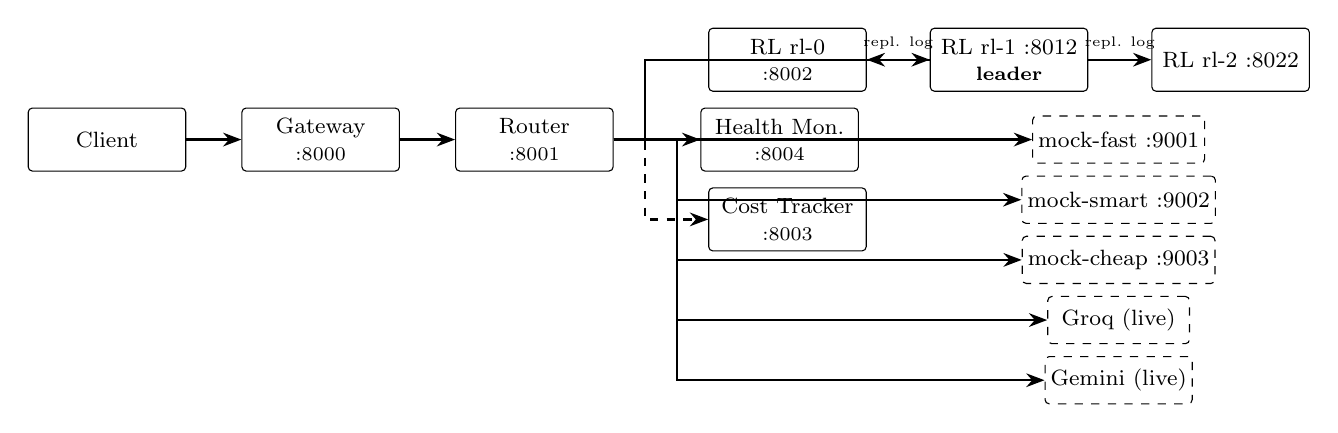
\begin{tikzpicture}[
  node distance=4mm and 7mm,
  font=\footnotesize,
  service/.style={rectangle, draw, rounded corners=1.5pt,
                  align=center, minimum width=20mm, minimum height=8mm,
                  inner sep=2pt},
  provider/.style={rectangle, draw, dashed, rounded corners=1.5pt,
                   align=center, minimum width=18mm, minimum height=6mm,
                   inner sep=2pt},
  arrow/.style={-Stealth, thick},
  asyncarrow/.style={-Stealth, thick, dashed},
]
  \node[service] (client) {Client};
  \node[service, right=of client] (gw) {Gateway\\\scriptsize :8000};
  \node[service, right=of gw] (router) {Router\\\scriptsize :8001};

  \node[service, above right=2mm and 12mm of router] (rl0)
    {RL rl-0\\\scriptsize :8002};
  \node[service, right=8mm of rl0] (rl1)
    {RL rl-1 :8012\\\scriptsize \textbf{leader}};
  \node[service, right=8mm of rl1] (rl2)
    {RL rl-2 :8022};

  \node[service, right=of router, xshift=4mm] (hm)
    {Health Mon.\\\scriptsize :8004};

  \node[service, below right=2mm and 12mm of router] (cost)
    {Cost Tracker\\\scriptsize :8003};

  \node[provider, right=22mm of hm] (mockf) {mock-fast :9001};
  \node[provider, below=1.5mm of mockf] (mocks) {mock-smart :9002};
  \node[provider, below=1.5mm of mocks] (mockc) {mock-cheap :9003};
  \node[provider, below=1.5mm of mockc] (groq)  {Groq (live)};
  \node[provider, below=1.5mm of groq]  (gem)   {Gemini (live)};

  \draw[arrow] (client) -- (gw);
  \draw[arrow] (gw) -- (router);
  \draw[arrow] (router.east) -- ++(4mm,0) |- (rl1.west);
  \draw[arrow] (router.east) -- (hm.west);
  \draw[asyncarrow] (router.east) -- ++(4mm,0) |- (cost.west);
  \draw[arrow] (router.east) -- ++(8mm,0) |- (mockf.west);
  \draw[arrow] (router.east) -- ++(8mm,0) |- (mocks.west);
  \draw[arrow] (router.east) -- ++(8mm,0) |- (mockc.west);
  \draw[arrow] (router.east) -- ++(8mm,0) |- (groq.west);
  \draw[arrow] (router.east) -- ++(8mm,0) |- (gem.west);

  \draw[arrow] (rl1) -- (rl0) node[midway, above, font=\tiny]{repl. log};
  \draw[arrow] (rl1) -- (rl2) node[midway, above, font=\tiny]{repl. log};

\end{tikzpicture}
\caption{IntelliRoute service topology. Solid arrows are synchronous
HTTP; dashed arrows are asynchronous fire-and-forget. Three
rate-limiter replicas form a single bully-elected cluster; the leader
serves all \texttt{/check} calls authoritatively and fans out a
replication log to the followers.}
\label{fig:arch}
\end{figure*}

\subsection{Intent Classification}
The router begins by classifying the request into one of four
intents: \texttt{INTERACTIVE}, \texttt{REASONING}, \texttt{BATCH}, or
\texttt{CODE}. We picked these four because they map cleanly to the
weight vectors we wanted to express in the ranker (latency-dominated
chat, capability-dominated reasoning, cost-dominated batch,
capability-and-latency code). The classifier itself is a deterministic
keyword/heuristic in \texttt{router/intent.py}, it scans the
joined message text for tokens like \texttt{def\,}, \texttt{import\,},
\texttt{Traceback}, \texttt{explain step by step}, \texttt{summarize
the following document}, etc. We deliberately avoided using a learned
model here because the distributed-systems contributions of the
project are not in classification, and a deterministic classifier
unit-tests cleanly without an external dependency. The classifier
also honors an optional client-supplied \texttt{intent\_hint} so
applications that already know their workload can skip the heuristic.

\subsection{Multi-Objective Routing}
Once an intent is known, the router asks the policy engine
(\texttt{router/policy\_engine/}) to apply pre-rank rules, batch
avoids premium providers, premium requires reasoning or a high
complexity score, tenant/team/workflow budget pressure can demote
premium-tier providers, brownout can block premium and prefer
low-latency providers, and an interactive latency gate filters out
providers whose declared p95 SLA exceeds the request's latency
budget. Each rule contributes audit metadata that is returned in a
\texttt{PolicyEvaluationResult} on the response, so we always know
\emph{why} a provider was filtered.

The surviving providers go into the multi-objective ranker
(\texttt{router/policy.py}). For each provider we compute four
sub-scores in $[0,1]$, latency, cost, capability, success rate,
and combine them using an intent-specific weight vector. The final
score is

\begin{equation}
S_p = w_L \cdot \tilde{L}_p + w_C \cdot \tilde{C}_p
    + w_K \cdot K_p + w_R \cdot R_p,
\label{eq:score}
\end{equation}

where $\tilde{L}_p$ and $\tilde{C}_p$ are min-max normalised
latency/cost values (lower is better, hence \emph{higher score}
better), $K_p$ is the provider's declared capability tier, and
$R_p$ is its EMA success rate from the feedback collector.
Table~\ref{tab:weights} shows the per-intent weight vectors we
shipped as defaults; the online \texttt{WeightTuner} in
\texttt{router/weight\_tuner.py} updates them at runtime as it
accumulates per-attempt outcomes.

\begin{table}[!t]
\caption{Default sub-score weights per intent. The online weight
tuner can rebalance these from observed outcomes.}
\label{tab:weights}
\centering
\renewcommand{\arraystretch}{1.1}
\begin{tabular}{lcccc}
\toprule
Intent       & $w_L$ & $w_C$ & $w_K$ & $w_R$ \\
\midrule
Interactive  & 0.55  & 0.15  & 0.20  & 0.10 \\
Reasoning    & 0.10  & 0.10  & 0.50  & 0.30 \\
Batch        & 0.05  & 0.65  & 0.15  & 0.15 \\
Code         & 0.10  & 0.05  & 0.65  & 0.20 \\
\bottomrule
\end{tabular}
\end{table}

\subsection{Distributed Rate Limiting}
The rate limiter is the part of the system where consistency matters
most. If we over-issue a token the application either incurs
unbudgeted spend or hits a 429 storm; either failure is hard to
unwind. We therefore run three replicas (\texttt{:8002},
\texttt{:8012}, \texttt{:8022}) with one leader. The leader owns the \texttt{TokenBucket} state and serves all
\texttt{/check} calls. Followers forward writes to the leader and
tail its replication log; if the leader cannot be reached, followers
fall back to local state by default, or fail closed when
\texttt{RATE\_LIMITER\_STRONG\_CONSISTENCY=1} is set. Each bucket is
keyed by \texttt{(tenant\_id, provider)} and resolves through a
layered configuration: exact pair, per-tenant any-provider,
per-provider any-tenant, then a global default.

Leader election is a bully-style protocol in
\texttt{rate\_limiter/election.py}. Replicas exchange
\texttt{/election/challenge}, \texttt{/election/victory}, and
\texttt{/election/heartbeat} messages, and the highest replica id
always wins. We picked bully over Raft for the same reason we picked
heuristics over a learned classifier: the goal of the project was to
make the consistency tradeoff visible and demonstrable, not to ship
a formally verified consensus implementation. Section~\ref{sec:limits}
discusses the implications of this choice.

\subsection{Circuit Breakers and the Fallback Chain}
The health monitor (\texttt{:8004}) runs a per-provider three-state
breaker (\texttt{closed} $\to$ \texttt{open} $\to$ \texttt{half\_open})
with a sliding error window of 20 outcomes, a default failure
threshold of 5, and a 10-second open-duration cooldown.
Figure~\ref{fig:breaker} sketches the state machine. On every
provider call, the router pushes a success/failure signal back to
the monitor via \texttt{/report/{provider}}. The monitor advances
\texttt{open} $\to$ \texttt{half\_open} \emph{lazily} when
\texttt{/snapshot} is read, this avoids a background thread per
provider and keeps the breaker side-effect-free between requests.

\begin{figure}[!t]
\centering
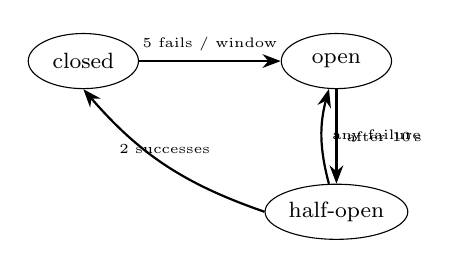
\begin{tikzpicture}[
  font=\footnotesize,
  state/.style={ellipse, draw, minimum width=14mm, minimum height=7mm,
                inner sep=1pt},
  arrow/.style={-Stealth, thick},
  node distance=12mm and 18mm,
]
  \node[state] (closed)   {closed};
  \node[state, right=of closed] (open) {open};
  \node[state, below=of open]   (half) {half-open};

  \draw[arrow] (closed) -- node[above, font=\tiny]
    {5 fails / window} (open);
  \draw[arrow] (open) -- node[right, font=\tiny]
    {after 10\,s} (half);
  \draw[arrow, bend left=15] (half.west) to node[above, font=\tiny]
    {2 successes} (closed.south);
  \draw[arrow, bend left=15] (half) to node[right, font=\tiny]
    {any failure} (open);
\end{tikzpicture}
\caption{Per-provider circuit breaker state machine.}
\label{fig:breaker}
\end{figure}

When the breaker for a candidate is open, the router skips it and
moves to the next provider in the ranked list. Retries against the
same provider use a jittered exponential back-off bounded by the
provider's declared p95 SLA, we did not want a slow provider's
back-off to consume the whole interactive latency budget. If
\emph{every} candidate trips out (open breakers, exhausted daily
quotas, denied by the rate limiter), the router returns a structured
HTTP 503 to the client rather than hanging.

\subsection{Brownout, Backpressure, and Priority Queueing}
Under sustained overload the system enters \emph{brownout}
(\texttt{router/brownout.py}). Four signals are tracked in a sliding
window: queue depth, p95 latency, error rate, and timeout rate. The
manager enters brownout when any of the four exceeds an enter
threshold for \texttt{enter\_consecutive} evaluations in a row, and
leaves only when all four sit below their exit threshold for
\texttt{exit\_consecutive} consecutive evaluations. We use this
hysteresis to avoid flapping between \texttt{normal} and
\texttt{degraded} on a single noisy sample.

While degraded, the system: (i)~drops or delays \texttt{LOW}-priority
requests, (ii)~blocks premium-tier providers for
\texttt{MEDIUM}/\texttt{LOW}, (iii)~prefers low-latency providers
even at higher cost, and (iv)~clamps \texttt{max\_tokens} for
\texttt{REASONING}/\texttt{BATCH}. The manager runs both globally
and per-tenant, so one noisy tenant cannot drag everyone else into
brownout.

The priority queue (\texttt{router/queue.py}) is the input side of
this. \texttt{INTERACTIVE} and \texttt{CODE} are \texttt{HIGH} and
bypass the queue entirely; \texttt{REASONING} is \texttt{MEDIUM};
\texttt{BATCH} is \texttt{LOW}. Above \texttt{shed\_threshold}, new
\texttt{LOW}-priority arrivals are shed instead of enqueued. Four
async worker tasks drain the queue.

\subsection{Cost Accounting and Budget Gates}
Cost events are published asynchronously from the router to the
cost tracker (\texttt{:8003}); the router does not wait for the
publish to succeed before returning the response. The accountant
maintains rollups at three scopes, tenant, team, workflow, and
exposes a pre-call gate \texttt{/budget/\{tenant\_id\}/check?
projected\_cost\_usd=...}. The router's \texttt{/complete} pipeline
calls the gate before sending the request, and demotes the head
candidate to the cheapest still-pending provider if the projected
cost would push past any active budget. This decision is logged with
the reason \texttt{budget\_gate\_demoted} in the trace ring buffer.

% =========================================================================
\section{Implementation Notes}\label{sec:impl}
% =========================================================================
The full system is approximately 8.7k lines of Python across the
\texttt{intelliroute/} package, plus the test suite. It runs on
Python 3.10+ with FastAPI and Uvicorn, talks HTTP between services
with \texttt{httpx}, and uses \texttt{pydantic} models as the wire
contract. There are no databases, no compiled extensions, and no
Docker requirements, a fresh clone runs end-to-end with
\texttt{pip install -e ".[dev]"} followed by
\texttt{python3 scripts/start\_stack.py}.

\subsection{Trace propagation and observability}
The gateway generates an \texttt{X-Request-Id} on every request and
propagates it to all downstream services. Every log line is JSON
(\texttt{intelliroute/common/logging.py}) and tagged with the
request id, so a single \texttt{jq} pipeline reconstructs the full
path of a request across services. The router additionally maintains
a 50-entry ring buffer of recent traces at \texttt{/traces} that the
dashboard polls. Figure~\ref{fig:flow} shows the synchronous and
asynchronous calls a single happy-path \texttt{/v1/complete} fans
out into.

\begin{figure}[!t]
\centering
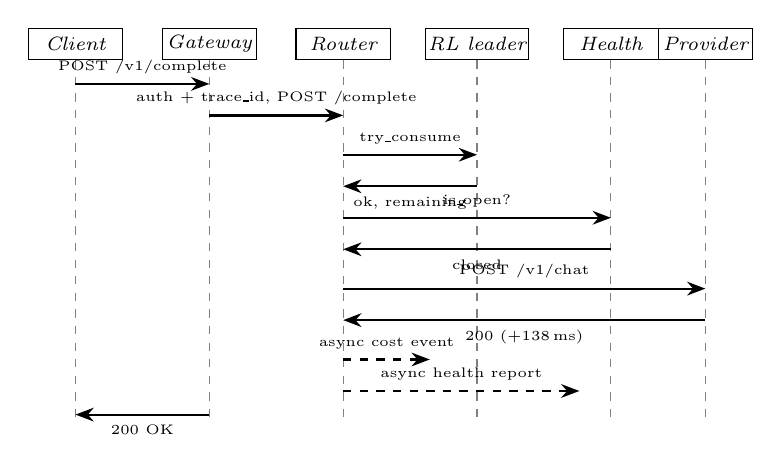
\begin{tikzpicture}[
  font=\scriptsize,
  arrow/.style={-Stealth, thick},
  asyncarrow/.style={-Stealth, thick, dashed},
  lane/.style={draw, minimum width=12mm, minimum height=4mm,
               inner sep=1pt, font=\scriptsize\itshape},
]
  \node[lane] (c)   at (0, 0)     {Client};
  \node[lane] (gw)  at (1.7, 0)   {Gateway};
  \node[lane] (r)   at (3.4, 0)   {Router};
  \node[lane] (rl)  at (5.1, 0)   {RL leader};
  \node[lane] (h)   at (6.8, 0)   {Health};
  \node[lane] (p)   at (8.0, 0)   {Provider};

  \foreach \n in {c,gw,r,rl,h,p} {
    \draw[gray, dashed] (\n.south) -- ++(0, -4.6);
  }

  \draw[arrow] ($(c.south)+(0,-0.3)$)
    -- node[above, font=\tiny]{POST /v1/complete}
       ($(gw.south)+(0,-0.3)$);
  \draw[arrow] ($(gw.south)+(0,-0.7)$)
    -- node[above, font=\tiny]{auth + trace\_id, POST /complete}
       ($(r.south)+(0,-0.7)$);
  \draw[arrow] ($(r.south)+(0,-1.2)$)
    -- node[above, font=\tiny]{try\_consume}
       ($(rl.south)+(0,-1.2)$);
  \draw[arrow] ($(rl.south)+(0,-1.6)$)
    -- node[below, font=\tiny]{ok, remaining}
       ($(r.south)+(0,-1.6)$);
  \draw[arrow] ($(r.south)+(0,-2.0)$)
    -- node[above, font=\tiny]{is\_open?}
       ($(h.south)+(0,-2.0)$);
  \draw[arrow] ($(h.south)+(0,-2.4)$)
    -- node[below, font=\tiny]{closed}
       ($(r.south)+(0,-2.4)$);
  \draw[arrow] ($(r.south)+(0,-2.9)$)
    -- node[above, font=\tiny]{POST /v1/chat}
       ($(p.south)+(0,-2.9)$);
  \draw[arrow] ($(p.south)+(0,-3.3)$)
    -- node[below, font=\tiny]{200 (+138\,ms)}
       ($(r.south)+(0,-3.3)$);
  \draw[asyncarrow] ($(r.south)+(0,-3.8)$)
    -- node[above, font=\tiny]{async cost event}
       ($(rl.south)+(-0.6,-3.8)$);
  \draw[asyncarrow] ($(r.south)+(0,-4.2)$)
    -- node[above, font=\tiny]{async health report}
       ($(h.south)+(-0.4,-4.2)$);
  \draw[arrow] ($(gw.south)+(0,-4.5)$)
    -- node[below, font=\tiny]{200 OK}
       ($(c.south)+(0,-4.5)$);
\end{tikzpicture}
\caption{Happy-path request flow for \texttt{POST /v1/complete}.
Solid arrows block the routing decision; dashed arrows are
fire-and-forget.}
\label{fig:flow}
\end{figure}

\subsection{Consistency model per data path}
The consistency model is summarized in Table~\ref{tab:consistency}.
Rate-limit checks are the only data path where we paid the cost of
strong consistency, because over-issuing tokens is the failure mode
that is hardest to undo. Cost rollups are the dual case, a few
seconds of staleness on a dashboard is fine, and an asynchronous
publish path lets the router stay on the request critical path.

\begin{table}[!t]
\caption{Consistency model per data path.}
\label{tab:consistency}
\centering
\renewcommand{\arraystretch}{1.15}
\setlength{\tabcolsep}{3pt}
\begin{tabularx}{\columnwidth}{@{}l l X@{}}
\toprule
Data path        & Model    & Why \\
\midrule
Rate-limit decisions & Strong    & Tokens are money; over-issue is
                                   hard to unwind. \\
Replication log      & Eventual  & Followers tail and replay so they
                                   can take over as leader. \\
Cost rollups         & Eventual  & Async events; small lag is fine. \\
Provider health      & Per-instance &
   Each health monitor maintains its own breaker state. \\
Service registry     & Per-router & In-process dict + lease TTLs;
                                   no cross-router sync. \\
Brownout state       & Per-router & Each router observes its own
                                   queue/p95/error window. \\
\bottomrule
\end{tabularx}
\end{table}

% =========================================================================
\section{Evaluation}\label{sec:eval}
% =========================================================================
We evaluated IntelliRoute along three axes: (i) a unit and integration
test suite, (ii) a deterministic replay harness that compares routing
policies under named scenarios, and (iii) a set of live failure-mode
demos.

\subsection{Test suite}
The repository ships with 259 tests across 28 \texttt{test\_*.py}
modules. 246 are unit tests against the pure components (token
bucket, breaker, election, intent classifier, ranker, accountant,
queue, brownout, weight tuner, registry, user feedback store). The
remaining 13 are end-to-end integration tests in
\texttt{tests/test\_integration.py} that spawn the full ten-process
backend on ephemeral ports and exercise it over real HTTP. The full
suite runs in roughly 12 seconds on a laptop, which is the single
fastest way we have found to confirm a fresh clone is healthy.

\subsection{Replay harness}
The replay harness (\texttt{intelliroute/eval\_harness/} +
\texttt{scripts/replay\_eval.py}, documented in
\texttt{docs/REPLAY\_EVAL\_HARNESS.md}) generates deterministic JSONL
workloads for four named scenarios and replays them against
\texttt{/v1/complete} while sweeping the router through five routing
policies. Before each \texttt{(scenario, policy)} run it resets all
mutable service state (router runtime, cost rollups, breakers, all
three rate-limiter replicas, mock fault flags) so cross-run
comparisons are fair. Per run it writes a \texttt{summary.json},
\texttt{metrics.csv}, \texttt{config.json}, \texttt{reset\_report.json},
\texttt{timeline.csv}, and \texttt{run.log} under
\texttt{artifacts/replay\_runs/}. The matrix run additionally writes
an \texttt{aggregate\_summary.json}, \texttt{run\_index.json}, and a
human-readable \texttt{report.md}. The metrics computed per
\texttt{(scenario, policy)} are total requests, success rate, error
rate, average / median / p50 / p95 / p99 latency, latency standard
deviation, total cost, average cost per request, premium usage rate,
fallback / reroute / reject counts, and provider distribution.
Table~\ref{tab:scenarios} summarizes the four scenarios.

\begin{table}[!t]
\caption{Replay scenarios.}
\label{tab:scenarios}
\centering
\renewcommand{\arraystretch}{1.15}
\setlength{\tabcolsep}{3pt}
\begin{tabularx}{\columnwidth}{@{}l X@{}}
\toprule
Scenario              & What it stresses \\
\midrule
\texttt{normal\_mixed} &
   Healthy baseline; mixed interactive/reasoning/batch load. \\
\texttt{degraded\_provider} &
   One provider degraded after reset; tests the failover and
   reroute paths. \\
\texttt{budget\_pressure} &
   Constrained tenant/team/workflow budgets force the policy to
   demote without full collapse. \\
\texttt{overload\_brownout} &
   Burst workload at high concurrency to trip the brownout
   manager. \\
\bottomrule
\end{tabularx}
\end{table}

\subsection{Live failure-mode demos}
Each mock provider exposes four fault-injection hooks
(\texttt{/admin/force\_fail}, \texttt{/admin/force\_timeout},
\texttt{/admin/force\_rate\_limit}, \texttt{/admin/force\_malformed})
plus a \texttt{/admin/reset} that clears them. The demo scripts
(\texttt{scripts/demo.py},
\texttt{scripts/demo\_failure\_recovery.py}) walk a breaker through
the full \texttt{closed} $\to$ \texttt{open} $\to$ \texttt{half\_open}
$\to$ \texttt{closed} cycle and print the snapshot at each step.
The leader-election failover demo is run by hand: identify the
current leader replica, kill its process, and observe the surviving
replicas elect a new leader within a few seconds.

% =========================================================================
\section{Limitations and Future Work}\label{sec:limits}
% =========================================================================
Several scoping decisions kept the project achievable in one
semester. Each is, in our view, a clean extension point rather than a
flaw.

\textbf{Bully-style election, not Raft.} Our election is a working
bully-style protocol with a replication log and follower
forwarding, enough to demonstrate the consistency-vs.-availability
tradeoff and enough to survive a leader kill. A formally verified
Raft implementation is the natural next step, especially because we
already have the log abstraction in place.

\textbf{In-memory state.} All in-memory state (rate-limit buckets,
breakers, registry, queue, brownout window, tuner weights) resets on
restart. Only user-feedback rows are persisted, in SQLite at
\texttt{artifacts/user\_feedback.sqlite3}. Swapping in Redis or
Postgres for the rest is a single-file change per subsystem because
the state is already encapsulated behind narrow interfaces.

\textbf{Heuristic intent classifier.} The classifier is a
keyword/heuristic in \texttt{router/intent.py}. We chose this so the
distributed-systems contributions could be unit-tested without an
external model, and so the demo would be deterministic. A small
fine-tuned classifier is the obvious upgrade, especially for prompts
where the keyword signals are ambiguous.

\textbf{Mock providers default in the demo.} The system ships
working Groq and Gemini adapters in
\texttt{router/provider\_clients.py}, but the demo defaults to mock
providers because they let us simulate latency, cost, and four
distinct failure modes without burning real-provider quota and
without a network dependency during grading.

\textbf{No cross-router state sharing.} The brownout window, the
weight-tuner state, and the service registry are all per-router. A
multi-router deployment would converge independently on each router.
Sharing this state across routers is a known unscoped item.

\textbf{Premium classification is heuristic.} ``Premium'' is decided
from the provider name pattern in the policy engine. A real
deployment would carry tier metadata from a provider catalog.

% =========================================================================
\section{Conclusion}
% =========================================================================
The 3 a.m. story we opened with is not really an LLM problem; it is
the absence of a control plane for traffic that should obviously
\emph{have} one. IntelliRoute is our argument, in code, that the same
distributed-systems machinery we already use for shared compute,
service discovery, leader election, replication, circuit breakers,
brownout, priority queueing, per-data-path consistency, applies
just as cleanly to the LLM fleet, and that wiring it together is a
one-semester project, not a multi-quarter platform investment. The
demo on the dashboard runs the full pipeline in roughly 140\,ms on a
laptop, the test suite runs in 12 seconds, and every concept we read
about in CMPE 273 maps to a specific module we can point at in the
source tree.

\end{document}
